\documentclass[10pt,journal,letterpaper,compsoc]{IEEEtran}
%
% If IEEEtran.cls has not been installed into the LaTeX system files,
% manually specify the path to it like:
% \documentclass[12pt,journal,compsoc]{../sty/IEEEtran}

% multirow
\usepackage{multirow}

% url
\usepackage{url}

% allow colors for inline comments
\usepackage{color}

% draw pictures with tikz package
\usepackage{tikz}
\usetikzlibrary{arrows, petri, topaths}
\usepackage{tkz-berge}



\ifCLASSOPTIONcompsoc

\else

\fi

\ifCLASSINFOpdf
\graphicspath{{images/}}
\DeclareGraphicsExtensions{.png}
\else

\fi

%
\usepackage{array}

%\hyphenation{op-tical net-works semi-conduc-tor}



\newcommand\TODO[1]{{\textcolor{red}{TODO:#1\\}}}
\begin{document}
%
% paper title
% can use linebreaks \\ within to get better formatting as desired
\title{Natural Language Interfaces to Structured Data}


\author{Author 1, Author 2, Author 3}





% The paper headers
\markboth{Journal of \LaTeX\ Class Files,~Vol.~6, No.~1, January~2007}%
{Shell \MakeLowercase{\textit{et al.}}: Bare Demo of IEEEtran.cls for Computer
Society Journals}

\IEEEcompsoctitleabstractindextext{
\begin{abstract}
Natural language interfaces to databases allow users to formulate queries in
natural language to databases. The benefits are twofold: first, users do not
have to know how the data have been modeled in the database, what term refers to
what database entity. Second, these systems can interface several data sources
that are possibly of different implementation and which data belong to different
domains.
In this paper we provide a survey of major natural language interfaces, from the
very beginning of artificial intelligence to most recent systems.
\end{abstract}

\begin{keywords}
Natural Language, Database
\end{keywords}}


% make the title area
\maketitle



\IEEEdisplaynotcompsoctitleabstractindextext



\IEEEpeerreviewmaketitle

%%%%%%%%%%%%%%%%%%%%%%%%%%%%%%%%%%%%%%%
%  INTRODUCTION                       %
%%%%%%%%%%%%%%%%%%%%%%%%%%%%%%%%%%%%%%%
\section{Introduction}
\label{sec:introduction}
Natural Language (NL) is the most natural and easy way to express information
need~\cite{Hearst:2011:NSU:2018396.2018414}. Moreover, it is not restricted to
experts who have a good knowledge on how to formulate a formal query.

NL as an interface has been investigated by researchers in both Information
Retrieval (IR) and Database communities. In the IR community however, the
keyword paradigm has become the most popular, for sure because of the success
of commercial search engines. 
%NL interfaces for unstructured documents are refered to as Question Answering
%(Q\&A) systems, that have received much researchers' attention as the Web had
Interfaces to unstructured documents has become popular as
the Web has made available huge amount of textual data, and recently as the
famous {\it Jeopardy!} quiz was won by IBM's {\sc
Watson}~\cite{FerrucciBCFGKLMNPSW10} system.
This trend seems to evolve slightly. For instance,
{\sc WolframAlpha}\footnote{\url{http://www.wolframalpha.com/}} is a popular
search service based on structured data, that accepts keyword queries as well
as some questions in natural language.

NL interfaces (to structured data) has focused much researchers' attention for
decades, but the field seems to have known a renewed interest for a few
years, probably thanks to the development of the semantic Web. 
Today's semantic technologies can be directly manipulated by experts, and
therefore there is still a need for interfaces. Indeed, users prefer NL
interfaces than the logic which is used in the semantic
Web~\cite{Kotov:2010:TNQ:1772690.1772746}.
However, the challenge of answering NL questions is far from being
solved~\cite{Kotov:2010:TNQ:1772690.1772746}.

NL interface: not only in the context of search (information retrieval), for
instance natural language query can be translated in goals / commands in the
context of (household) appliances (see {\sc
Exact}~\cite{Yates:2003:RNL:604045.604075}, not surveyed here).



In this survey, we outline the major dimensions of existing systems
and present the new trends and challenges of state-of-the-art systems.
The history of NL interfaces can be developped as follows:
\begin{enumerate}
  \item early years of domain-specific systems
  \item complex question answering in a specific domain
  \item rise of domain awareness in NL interfaces (through learning techniques)
  \item data-driven systems with respect to
  \begin{itemize}
    \item resources: almost domain-independent systems
    \item large-scale data: domain-independent systems
  \end{itemize}
\end{enumerate}
We present section~\ref{sec:main-dimensions} the main dimensions used throughout
the paper. 










%%%%%%%%%%%%%%%%%%%%%%%%%%%%%%%%%%%%%%%
% BIG PICTURE                         %
%%%%%%%%%%%%%%%%%%%%%%%%%%%%%%%%%%%%%%%
\section{Main Dimensions}
\label{sec:main-dimensions}
In this section, we introduce the main dimensions based on which NLI approaches
can be distinguished. The input to every NLI is the (1)~\emph{data}, and
(2)~\emph{user questions} representing information needs, which are translated
to an (3)~\emph{internal representation} of the needs employed by the system
and/or directly mapped to (4)~\emph{database queries} that finally, are
executed by the underlying query engine to produce the final answers. The main
problem tackled by a NLI approach is to transform the question to the internal
representation and then to the database query (2 $\mapsto$ 3 $\mapsto$ 4), or
to directly mapped the question to the query (2 $\mapsto$ 4). This problem is
hard when considering the large and rapidly evolving mass of structured data
that have become available. The major challenges modern NLI systems are facing
in this regard is to operate across domains (5)~\emph{domain-independence} as
well as to adopt to new domains (6)~\emph{portability}. For evaluating the
quality of the NLI output, different (7)~\emph{metrics} based on the user
questions the system can understand as well as the database queries it can
produce, have been proposed.

\TODO{old content that might be considered:} 
Dimensions:
\begin{itemize}
  \item What kind of query? (NL, controlled language)
  \item What are the data? 
  \item Target structured query: select query? update query?
  \item What are the answers?
  \item How portable is the system? Does it improve its performance over time?
  \item What is the linguistic coverage of the system? 
  \item Error feedback: how well is the user informed of misunderstanding of her
  question
  \item Predictability: how the system disambiguates / lets the user decide what
  should be the correct interpretation
  \item Performance: response time / evaluation metrics
\end{itemize}



\subsection{Data}
\label{sec:data}
%\TODO{Discuss the different types of structured data models that have been
% used, make clear that while they vary in expressiveness, they commonly enables
%capturing resources/entities/objects and relationships between them. Besides
%domain information captured in terms of entities and relationships, also point
%out other popular types of information that have considered, e.g. temporal and
%spatial information}

There is a great variety of structured data sources:
\begin{itemize}
  \item early data structures (Prolog databases; hierarchical lists)
  \item relational databases
  \item XML databases
  \item ontologies; \emph{linked data}
\end{itemize}
Structures of these data sources are different, as well as the way to access and
modify data (i.e. how to query data, which language to use, etc.).
For example, relational databases are represented with the entity/relationship
model and queries are usually expressed in a SQL-like language. Hierarchical
lists are hierarchical structures (like XML documents) that are composed of
embeded key-value pairs with optional attributes. XML documents are more
generic, since ``keys'' in those documents are nodes (i.e. can be trees
themselves). 
Ontologies are not more generic than XML databases from the structure point of
view, but allow to express easily semantic relationships.

Dome data structures are dedicated to some types of information. For instance,
temporal databases are similar to relational databases, but capture \emph{time}
in addition. Indeed, in some domains, the truth value of a fact or of
a resultset is determined by a \emph{timestamp}, while in classic database facts
are true in general. 

At the end, all these data structures manipulate \emph{entities} (i.e. named
properties of the database) and \emph{relations} between these entities.
Any database selection query can be reduced to a set of constraints on these
entities and relations. 





\subsection{Users' questions}
%\TODO{Discuss different types user questions}

\label{sec:big-picture-question}
Traditional database management systems provide an interface that allows users
to query the data in a formal language (e.g., SQL).

Question typing is a research task within the Q\&A field.
This community has classified questions in \emph{facto\"id questions} (i.e.
questions that can be answered by an \emph{objective} fact, typically questions
staring with wh-words except ``why'') and \emph{complex questions} which
answers are usually \emph{subjective} to the answerer, and for which there
might be several \emph{true} answers, possibly contradicting each other.
Complex questions can be ``why''-questions, ``how''-questions or
\emph{definition}-questions.
Facto\"id question is defined by Soricut \&
Brill~\cite{Soricut:2006:AQA:1127331.1127342} as questions ``for which a
complete answer can be given in 50 bytes or less, which is roughly a few
words'' (see also Kwok et al. ``Scaling question answering to the Web, WWW).
Several finer classification have been proposed in specific domains or
applications. 
For instance, in the case of temporal questions, Saquete et
al.~\cite{Saquete:2004:SCT:1218955.1219027} have proposed the classification
reproduced table~\ref{tab:saquete-classification}.
\begin{table}
\centering
\begin{tabular}{ll}\hline
\multicolumn{1}{c}{\textbf{Question type}} &
\multicolumn{1}{c}{\textbf{Example}}\\\hline\hline
Single event temporal questions &
``When did Jordan close \\
 without temporal expressions & the port of Aqaba to Kuwait?''\\\hline 
 Single event temporal questions & 
``Who won the 1988 New \\
 with temporal expressions & Hampshire republican primary?''\\\hline
 \multirow{2}{*}{Multiple events temporal questions} & ``What did G. Bush do
 after\\
  & the U.N. Security Council\\
 \multirow{2}{*}{with temporal expressions} & ordered a global embargo on\\
  & trade with Irak in August 90?''\\\hline
  \multirow{2}{*}{Multiple events temporal questions} & ``What happened to world
  oil\\
   & prices after the Iraqi\\
  without temporal expressions & annexation of Kuwait?''\\\hline
 
\end{tabular}
\caption{Question classification for temporal databases from~\cite{Saquete:2004:SCT:1218955.1219027}}
\label{tab:saquete-classification}
\end{table}

\subsubsection{Keyword query}
A {\it keyword query} consists in a set of words
traditionally used in the context of document search (i.e. searching relevant
documents given a textual query).
The classic idea is to represent documents in a vector model, where the vector
is composed of terms of documents. Search engines have made this paradigm
popular.
Hearst~\cite{Hearst:2011:NSU:2018396.2018414} reports that the number of words
in queries over Web search engines trends to increase (the experiment compared
queries performed over a month in 2009 and in 2010): queries from 5 to 8 words
increase up to 10\% while queries from 1 to 4 words decrease up to 2\%.
It seems indeed that users are more and more aware of new capabilities of
state-of-the-art search engines, and are less reluctant to express their
information need in a more ``natural'' way.

\subsubsection{Natural language query}
Early systems understood some English words and English syntactic constructions;
such language was called ``English-like'' by
authors~\cite{Woods:1973:PNL:1499586.1499695}. More recent systems try to go
further and to capture as much as possible the regularities as well as the
irregularities of NL.

Current systems handle only a subset of NL questions (the questions that the
system can understand). This ``subset'' of NL is called controled NL. Some
systems even go further, and are able to analyze why a question can not be
answered. It could be out of coverage of linguistic understanding of the system
(the question is not understood) or cannot be answered because the knowledge
base does not contain the answer (even if the semantics of the question is
fully captured).

Users prefer NL questions than keywords~\cite{Hearst:2011:NSU:2018396.2018414}.
In this survey, we focus on natural language interfaces, and not on keyword
search over structured data, even if the latter has become more popular
lately\footnote{Paper to be published at VLDB 2012: ``SODA: Generating SQL for
Business Users'' from Blunschi et al.: Keyword-based interface to data
warehouses}.




\subsection{Internal representation}
\label{sec:big-picture-syntactic}

Syntactic question representation (also called {\it parse tree} because the
tree graph structure is used most of the time) is an intermediate
representation, before the creation of the internal semantic representation. In
lots of systems, however, the syntactic representation also contain semantic
pieces of information: nodes of the syntactic tree contain information about how
to generate fragments of the target database query. 
The nodes of the tree representation contain information about words and
relations between words of the question. 
Typical semantic information contained in a syntactic parse tree are the
database elements that those words refer to. 
Those semantic information (also referred to as ``meaning'' in early systems)
are kept in a lexicon. 
The syntactic parse tree usually does not try to resolve
ambiguities, and keep all possible interpretations. Resolution of ambiguities
is done afterward, when building the semantic representation out of the
syntactic representation.







\subsection{Database queries}
\label{sec:big-picture-semantic}
%\TODO{Discuss query languages; discuss the different types of queries expressed
%by these languages, e.g. entity queries, relational queries, additional
%constructs such as group by etc.}

\begin{table*}[h!]
\centering
\begin{tabular}{|c|c|c|}\hline
{\bf System} & {\bf Internal representation} & {\bf DB query}\\\hline\hline
{\sc Baseball}~\cite{Green:1961:BAQ:1460690.1460714} & specification list &
$\surd$\\\hline
{\sc Lunar}~\cite{Woods:1973:PNL:1499586.1499695} & meaning representation
language & X\\\hline 
{\sc Chat-80}~\cite{Warren:1982:EEA:972942.972944} &
logic expression & X\\\hline
{\sc Team}~\cite{Grosz:1987:TED:25672.25674} & logic expression & X\\\hline
{\sc Qwerty}~\cite{Nelken:2000:QTD:992730.992808} & logic expression & X\\\hline
{\sc Irus}~\cite{Bates:1983:IRU:511793.511804} & meaning representation language
& X\\\hline
{\sc Precise}~\cite{Popescu:2003:TTN:604045.604070} & graph representation &
X\\\hline
{\sc Masque/SQL}~\cite{Androutsopoulos93masque} & meaning representation
language (LQL) & X \\\hline 
{\sc NaLIX} \& {\sc
DaNaLIX}~\cite{Li:2005:NIN:1066157.1066281,Li:2007:DDN:1247480.1247643} & XQuery
& $\surd$\\\hline 
{\sc C-Phrase}~\cite{Minock:2010:CSB:1715942.1716190} & $\lambda$-calculus & X
\\\hline
{\sc Panto}~\cite{Wang:2007:PPN:1419662.1419706} & graph representation (query
triples) & X\\\hline 
{\sc Orakel}~\cite{Cimiano:2007:PNL:1216295.1216330} & $\lambda$-calculus &
X\\\hline
Miller et al.~\cite{Miller:1996:FSA:981863.981871} &
semantic frames & X\\\hline 
Zettlemoyer et
Collins~\cite{DBLP:conf/uai/ZettlemoyerC05} & $\lambda$-calculus &
$\surd$\\\hline 
{\sc Wolfie}~\cite{Thompson:2003:AWM:1622420.1622421} & Prolog & $\surd$
\\\hline {\sc PowerAqua}~\cite{DBLP:conf/esws/LopezMU06} & graph representation
(query triples) & X\\\hline
{\sc DeepQA}~\cite{FerrucciBCFGKLMNPSW10} & semantic triples & $\surd$\\\hline
\end{tabular}
\caption{Semantic meaning representations}
\label{tab:semantic-meaning-representation}
\end{table*}

The parse tree (which may or not contain semantic information in parse tree
nodes) must then be {\it interpreted} in some internal semantic representation.
Table~\ref{tab:semantic-meaning-representation} displays semantic meaning
representations used in different systems.
As shown in this table, the internal semantic representation can be or not the
targetted query representation. 
The expressivity of the database query is discussed in section
section~\ref{sec:big-picture-expressivity}. 
The semantic representation is intented to capture as much as possible users'
intent, and is sufficient to generate the final database query. 
While the syntactic representation may contain lots of ambiguities, the semantic
representation does not. 
The semantic representation depends on the data structure. However, to
demonstrate their portability features, some systems contain components that
can translate the semantic representation for different database query
languages.

\subsubsection{Query languages}
Relational databases are generally associated with the SQL query language (and
temporal databases are associated to an extension of SQL called temporal SQL).
Multidimensional databases (e.g., data warehouses) are associated with MDX,
which is a SQL-like query languages dedicated for handling measures, dimensions
and hierarchies (key concepts of multidimensional models).
Other data stuctures are associated with their own query language. For instance,
hierarchical lists (or specification lists) is not associated with a language,
but to a similar structure, which is a template where empty slots correspond to
the expected items of the resultset. XML databases are associated to XPath, and
semantic databases (e.g., RDF) are usually queried with languages derived from
SPARQL which looks similar to SQL.
Recently, new query languages have appeared (``no-SQL''). 
\TODO{Develop\ldots}

\paragraph{Selection}
\label{sec:query-languages-selection}
a selection consists in choosing the expected database attribute to appear in
the resultset.
In SQL, the selection is expressed as \verb?SELECT t.x?, where $t$ is a table
and $x$ a field or attribute belonging to $t$. In SPARQL it corresponds to
\emph{variables} that are defined in the query, and that must satisfy the
constraints defined in the \verb?WHERE? section of the SPARQL query (see
section~\ref{sec:query-languages-constraints}).
In MDX, the selection corresponds to the ordered set of dimensions or measures
that should appear in the resultset, with the information about the level of the
expected attributes in the hierarchy, and the filters. For instance,
\verb?SELECT Country.[All members]? corresponds to the selection of the
dimension ``Country'' with no filter (i.e. selection of all members of the
dimension ``Country'').
Selection for a hierarchical list corresponds to a slot in the structure
template.
A selection in a XPath query corresponds to\ldots\footnote{\TODO{Find what}}
In SPARQL, a selection can be expressed also differently. Indeed, the output of
a SPARQL query can be a data structure of the same kind than the data themselves
(i.e. a graph). This is performed with the \verb?CONSTRUCT? keyword.

\paragraph{Constraints}
\label{sec:query-languages-constraints}
Canstraints in database queries aim at reducing the size of the resultset.
In the case of SQL, SPARQL and MDX, such constraints are introduced with the
\verb?WHERE? keyword. For SQL, these constraints can define how different tables
can be \emph{joined} together such that attributes belonging to different tables
can appear in a single view (i.e. in the resultset). Other kinds of constraints
are about the values of attributes.
For SPARQL, the constraints are expressed with \emph{triples} (which can be
made of some \emph{blank node} or undefined node). Thus, a SPARQL constraint is
about relations between entities (see \emph{joins} for relational databases), or
about entities themselves (which type must be the entity? If this is a
\emph{litteral}, in what range of value must it belong?,etc.).



\paragraph{Query modifiers}
\label{sec:query-languages-modifiers}
Conceptually, modifiers are primitives that modify the resultset afterwards.
Such primitives can - order the resultset along a given attribute (e.g.,
\verb?ORDER BY? in SQL); - select at most $n$ \emph{tuples} of the resultset
(e.g., \verb?LIMIT x? in SQL); - select only different tuples (e.g., the
keyword \verb?DISTINCT? in SQL).
In SPARQL, it is possible to test if a set of constraints can be satisfied from
the data, and to combine these tests with optional constraints (\verb?OPTIONAL?
keyword) or mandatory constraints (\verb?FILTER? keyword).





\subsubsection{Expressivity of database query}
\label{sec:big-picture-expressivity}



%\subsection{Results}
%\label{sec:big-picture-results}

NL interfaces produce database queries.
Those queries must be then be executed by underlying DBMS.
The execution of queries can lead to different failing states:
\begin{itemize}
  \item the query execution fails (the generated database query is not valid)
  \item the query execution lead to an empty result set
\end{itemize}
In these cases, the system may inform the user and/or suggest/rephrase the
query. This is especially performed in systems belonging to the feedback
approach (see section~\ref{sec:feedback-driven}). 


\subsection{Domain-independence}
\label{sec:main-dimensions-domain-independance}
Domain-independance is the ability of a system, to operate accross different
domains simultaneously. 
In practice, this means that a domain-independant system would be on top of
different data sources that belong to different domains, and that this system is
able to meet users' requests for any of these domains. 
The main difficulty of building domain-independant systems is the ability to
translate NL constructions differently in the different application domains.
For instance, the qualitative expression ``middle-aged'' can be interpreted
completely differently accross the different domains.


\subsection{Portability}
\label{sec:main-dimensions-portability}
A system is said \emph{portable} if it can be easily configured for different
domains (than the domain for which it was first designed).
Domain-independance (section~\ref{sec:main-dimensions-domain-independance}) is a
step further, because different domains are considered simultaneously; while in
portable systems the challenge is to ease the configuration.
Portable systems are also referred to as \emph{configurable} interfaces in the
following.
Configurable interfaces let users improve the system's capabilities, both the
linguistic coverage $S$ and the system coverage $K$ (see
Fig.~\ref{fig:interface}).


Minock et al.~\cite{Minock:2010:CSB:1715942.1716190} have identified three kinds
of configuration applicable to NL interfaces:
\begin{itemize}
  \item let users name database elements, so that phrases used in the question
  can be easily mathed with database elements
  \item offer a GUI that generates automatically semantic rules or a grammar for
  translating NL questions to database queries
  \item use machine learning techniques to induce semantic rules or a grammar
  from annotated corpora
\end{itemize}
These ways of configuring interfaces are not equally costly: for instance, the
third one (machine learning techniques) can be highly costly if it requires a
huge volume of annotated data. The cheapest configuration is based on user
interaction, where no initial configuration is needed, but domain-specific
knowledge is learned based on user interaction. An example of such a
system is {\sc NaLIX}~\cite{Li:2005:NIN:1066157.1066281}.




\subsection{Metrics}
\label{sec:big-picture-metrics}
Several evaluation metrics have been introduced in various systems. We review
them briefly below.
We present the interesting figure~\ref{fig:interface} copied from Han et al.
work~\cite{Han:2010:NLI:1719970.1720022}. It shows the tradeoff between
linguistic coverage (``Expressions interpretable by a System'') and the
expressions that can be answered from a knowledge base. The goal of any
interface would be that the linguistic coverage comprises all expressions that
can be answered by the knowledge base.

 \begin{figure}[!h]
\centering
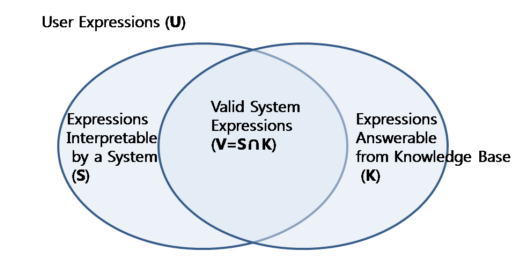
\includegraphics[width=8cm]{images/interface}
\caption{Linguistic coverage vs. logical coverage within interfaces, copied
from~\cite{Han:2010:NLI:1719970.1720022}}
\label{fig:interface}
\end{figure}

\subsubsection{Fluency$_{Woods}$}
Woods~\cite{Woods:1973:PNL:1499586.1499695} defines {\it fluency} as ``the degree
to which virtually any way of expressing a given request is acceptable''.
Fluency measures roughly how easy to use is a system. 
Intuitively, a good fluency means a ``natural'' interface in the sense of
natural interfaces~\cite{Hearst:2011:NSU:2018396.2018414}. This requires
advanced natural language techniques, and would probably lead to systems that
can interpret more expressions than those that can be actually answered by the
knowledge base ($S\setminus K$ in figure~\ref{fig:interface} would not be
negligeable).
 

\subsubsection{Completeness$_{Woods}$}
{\it Completeness} was first defined in Woods' work related to the {\sc
Lunar}~\cite{Woods:1973:PNL:1499586.1499695} system. 
It measures if there is a way of expressing any query which is logically
possible from the database. In the end, it measures if the interface can answer
all possible questions. In figure~\ref{fig:interface}, completeness would be
represented by $S$ comprising $K$ ($K\subset S$).


\subsubsection{Soundness$_{Popescu}$}
An interface is said {\it sound} if ``any SQL output is a valid interpretation
of the input English sentence''~\cite{Yates:2003:RNL:604045.604075}. In
figure~\ref{fig:interface}, this evaluates the expressions of $V=S\cap K$.


\subsubsection{Completeness$_{Popescu}$}
An interface is said {\it complete} if it ``returns all valid interpretations of
input sentences''~\cite{Yates:2003:RNL:604045.604075}.
Yates et al. have reused this metrics in their {\sc Exact} system (not surveyed
here). They do not claim that users should restrict their questions to query
only tractable qestions; but they suggest that identifying classes of questions
that are semantically tractable and measuring the prevalence of these questions
is the direction of current research.


\subsubsection{User's intent}
Yates~\cite{Yates:2003:RNL:604045.604075} makes an assumption, that if the
interface is sound, complete and if a single SQL statement can be produced from
a NL question, then the interface has unambiguously determined user's intent. 

\begin{figure*}
\centering
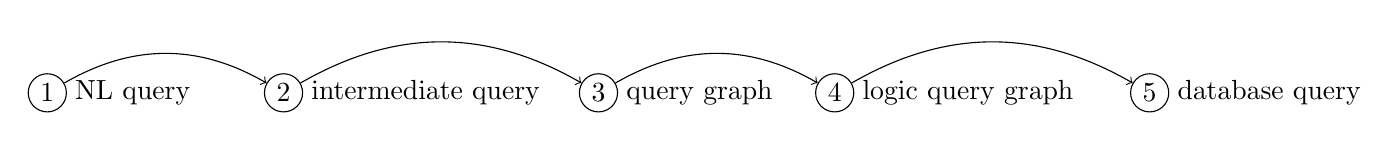
\begin{tikzpicture}[transform shape]
%\tikzset{VertexStyle/.append style = {minimum size = 3pt}}
\node at (0,0) [draw,circle,inner sep=2pt](1){1};
\node at (3,0) [draw,circle,inner sep=2pt](2){2};
\node at (7,0) [draw,circle,inner sep=2pt](3){3};
\node at (10,0) [draw,circle,inner sep=2pt](4){4};
\node at (14,0) [draw,circle,inner sep=2pt](5){5};
\node at (0,0) [draw=none,fill=none,label={[label distance=3pt]0:{NL query}}]
{}; 
\node at (3,0) [draw=none,fill=none,label={[label
distance=3pt]0:{intermediate query}}] {}; 
\node at (7,0) [draw=none,fill=none,label={[label
distance=3pt]0:{query graph}}] {};
\node at (10,0) [draw=none,fill=none,label={[label
distance=3pt]0:{logic query graph}}] {};
\node at (14,0) [draw=none,fill=none,label={[label
distance=3pt]0:{database query}}] {};
\draw[->](1) edge[bend left] (2);
\draw[->](2) edge[bend left] (3);
\draw[->](3) edge[bend left] (4);
\draw[->](4) edge[bend left] (5);
\end{tikzpicture}
\caption{Big picture of NLI systems}
\label{fig:big-picture}
\end{figure*}

\subsubsection{Predictability}
Within user interfaces, predictability has been pointed out as the essential
feature of user interfaces in the 90' by
Norman~\cite{Norman:1994:MPI:176789.176796} and Schneiderman et
Maes~\cite{Shneiderman:1997:DMV:267505.267514}. 
Predictability and the feel of control seems however to be in contradiction with
personalization, which is the one pillar of recent IR systems. 
















%%%%%%%%%%%%%%%%%%%%%%%%%%%%%%%%%%%%%%%
% ANATOMY OF SYSTEMS                  %
%%%%%%%%%%%%%%%%%%%%%%%%%%%%%%%%%%%%%%%
\section{Anatomy of NLI systems}
\label{sec:anatomy}
The main problem to solve is to map user's intent expressed in a natural way
(say unstructured way) to a database query, which is a structured expression
where there is no room for ambiguity unlike natural language. The problem that
NLI systems try to solve, is equivalent to finding a mapping $f$ between natural
language questions $q$ and families of structured queries $(q^\prime_i)_i$
(where the index corresponds to the \emph{rank} of the structured query):
\begin{equation}
f:\left\{
\begin{array}{l}
Q\rightarrow (Q^\prime)^I\\
q\mapsto(q^\prime_i)_i
\end{array}\right.
\end{equation}
where $i\in I=[0,n]$ is the index of $q^\prime_i$.
 


\subsection{Lexicon}
The lexicon is a data structure that is used to reduce the ambiguity in words
when analyzing users' questions. 
NLI are usually composed of two lexicons: a domain-dependant lexicon and a
domain-independant lexicon. 
The domain-dependant lexicon defines words in terms of semantic rules (see
section~\ref{sec:anatomy-semantic-rules}).
The domain-independant lexicon defines how to interpret words independant from a
given domain. For instance, {\it wh}-question words define constraints on the
structure of the expected database query (for SQL, for the ``WHERE'' statement
for instance). 



\subsection{Semantic rules}
\label{sec:anatomy-semantic-rules}
Semantic rules define the semantics of question words. The input in a node, or a
part of the parse tree being constructed, and the output contains information on
how to construct part of the final database query. The final database query will
be generated from the parse tree, which contains semantic information in the
nodes, in addition to lexical and syntactic information. 
The idea behind this process is a linguistic theory [missing ref], where the
global meaning of a sentence is defined by the individual meanings of words /
expressions in the sentence, and by the syntactic relationships between the
words / phrases. 




\subsection{Main problems to solve}
The main problems to solve:
\begin{itemize}
  \item have the boroadest linguistic coverage (let users use their own
  terminology)
  \item mechanisms that permit to query other domains with a low porting cost
  \item ensure that the resulting database query is valid
\end{itemize}









%%%%%%%%%%%%%%%%%%%%%%%%%%%%%%%%%%%%%%%
% OVERVIEW SECTION                    %
%%%%%%%%%%%%%%%%%%%%%%%%%%%%%%%%%%%%%%%
\section{Taxonomy of main approaches}
\label{sec:overview}




\textbf{Classic translation approach}
The classic translation approach consists in going from (1) to (4).
To reach step (3), semantic rules are needed to find out what database elements
should be associated to question phrases. 

\textbf{Iterative approach}
The iterative approach does not go directly from (1) to (3), but goes back to
(1) several times before reaching step (3). 
Those iterations correspond to question reformulations, that involve
user-feedback to interpret semantically the question in terms of a database
query.


The way translation from NL questions to formal query has evolved over years.
Table~\ref{tab:overview} presents an overview of major systems that we consider
in the survey.

\begin{table*}
\centering
\begin{tabular}{|c|c|c|c|c|c|c|c|}\hline
%\begin{tabular}{|c|c|c|c|c|c|c|c|}\hline
\multirow{2}{*}{\bf Approach} & \multirow{2}{*}{\bf System} &
\multicolumn{6}{c|}{\bf Dimensions}\\\cline{3-8}
& & {\bf Query} & {\bf Data} & {\bf Answers} & {\bf Portability} & {\bf
Linguistic coverage} & {\bf Error feedback}\\\hline\hline 
\multirow{2}{*}{Domain-dependent semantic parsing} & {\sc
Baseball}~\cite{Green:1961:BAQ:1460690.1460714} & & & & & & \\\cline{2-8}
& {\sc Lunar}~\cite{Woods:1973:PNL:1499586.1499695} & & & & & & \\\hline
\multirow{5}{*}{Complex question translation} & {\sc
Chat-80}~\cite{Warren:1982:EEA:972942.972944} & & & & & & \\\cline{2-8}
& {\sc Irus}~\cite{Bates:1983:IRU:511793.511804} & & & & & & \\\cline{2-8}
& {\sc Qwerty}~\cite{Nelken:2000:QTD:992730.992808} & & & & & & \\\cline{2-8}
& {\sc
Precise}~\cite{Popescu:2004:MNL:1220355.1220376,Popescu:2003:TTN:604045.604070}
& & & & & & \\\cline{2-8}
& {\sc Panto}~\cite{Wang:2007:PPN:1419662.1419706} & & & & & & \\\hline
\multirow{5}{*}{Feedback-driven approaches} &
{\sc Masque/SQL}~\cite{Androutsopoulos93masque} & & & & & & \\\cline{2-8}
& {\sc Team}~\cite{Grosz:1987:TED:25672.25674} & & & & & & \\\cline{2-8}
& {\sc NaLIX} \& {\sc DaNaLIX}~\cite{Li:2005:NIN:1066157.1066281} & & & & & &
\\\cline{2-8}
& {\sc C-Phrase}~\cite{Minock:2010:CSB:1715942.1716190} & & & & & &
\\\cline{2-8}
& {\sc
Orakel}~\cite{Cimiano:2007:PNL:1216295.1216330} & & & & & & \\\hline
\multirow{3}{*}{Learning-based approaches} & Zettlemoyer
et al.~\cite{DBLP:conf/uai/ZettlemoyerC05} & & & & & & \\\cline{2-8}
& Miller et al.~\cite{Miller:1996:FSA:981863.981871} & & & & & & \\\cline{2-8}
& {\sc Wolfie}~\cite{Thompson:2003:AWM:1622420.1622421} & & & & & &
\\\hline
\multirow{2}{*}{Schema-unaware approaches} & {\sc
PowerAqua}~\cite{DBLP:conf/esws/LopezMU06} & & & & & & \\\cline{2-8}
 & {\sc DeepQA}~\cite{DBLP:journals/aim/FerrucciBCFGKLMNPSW10} & & & & & &
 \\\hline
\end{tabular}
\caption{Overview of major NL interfaces to structured data}
\label{tab:overview}
\end{table*}

\subsection{Domain-dependent semantic parsing}
Early systems belong to this class of approaches.
The knowledge necessary to translate NL questions to database queries
is encoded in lexicon.
The systems allows users to use a subset of English (controlled language) to
query databases. 
The lexicon, however, is a huge linguistic resource which defines how each word
must be translated into database elements, and what semantic rules to trigger to
get, in the end, the desired database query.



\subsubsection{Lexicon}
The lexicon is a resource that ``defines'' a set of words that belong to a
domain. Those words are associated to a ``meaning'', which is a semantic rule
that says how this word must be interpreted in the data domain and given
the data structure.
In addition, the lexicon also contains a list of specific rules that modify 
the global meaning of the sentence, given some words that are already defined in
the lexion.
The lexicon usually combines both syntactic with semantics information.
For instance, the same word would have a different interpretation if it's a noun
or a verb in a sentence. 

\subsubsection{Limitation}
The domain dependence is however the great limitation of those systems; this is
due to the cost of the lexicon. Indeed, porting such systems to other domain
would mean provide a new lexicon and corresponding semantic rules, which is
highly costly.


 







\subsection{Complex question translation}
The next generation of NL interfaces aims at increasing the linguistic coverage.
This is performed with the distinction of both domain-dependent knoweldge and
domain-independent knowledge.
The domain-dependent knowledge base consists in semantic rules triggered by
words, phrases or syntactic information encoded in a parse tree. Those rules
produce fragments of the target query language (or of the intermediate query
language) to be then combined and modified to generate the final qurey language.
The domain-independent knowledge base is composed of lexical information in a
dictionary (which might be completed with domain-dependent knowledge, like the
most likely senses of words used in the application domain).







\subsection{Feedback-driven approaches}
This range of systems translate NL questions to database queries basing on
users' feedback. 
We distinguish between the following kinds of feedback:


\subsubsection{Authoring tool configuration}
Authoring tools are GUI that permits users to edit domain-specific knowledge
(e.g., the lexicon that is used to translate NL questions to internal queries). 
Domain-specific knowledge edited within such tools can be straightforward (like
synonyms to be used in user's question to describe the same database elements)
or more complex like semantic rules to translate user's terms to logical
elements.
Describing this knowledge is not an easy task for standard users, for instance
semantic rules that define how to map words/phrases to logical elements, and
rules that define how information from the parse tree must be combine to
produce the final logical query.
For that reason, recent advanced systems try to infer such rules basing on
dialog-like interaction. 


\subsubsection{Interactivity}
Authoring tools presented in the previous section are intended to be used as a
preliminary task when porting the interface to other domains. 
Other systems do not explicitely ask users to answer question to get the
domain-specific knowledge, but infer this knowledge basing on interaction when
using it. 
This range of systems suggests users NL questions that could be reformulations
of the current user's question. 
To the best of our knowledge, there are two different kinds of such interaction,
when the system cannot interpret a question:
\begin{itemize}
  \item the system tries to change words/phrases in user's question, so that the
  system is able to interpret the question
  \item the system also comprises a repository of successfully answered
  questions, and suggests one of those questions replacing some slots with terms
  used in the user's question, and ensuring that the generated question can be
  interpreted by the system
\end{itemize}
Recent work~\cite{DBLP:conf/icde/KoutrikaSI10} investigate how to present
similar questions in NL as interpretations of the current question. 
This is a way of making the user think she controls what is happening, which is
one of the features of modern interfaces. 
This paraphrasing feature is also present in {\sc NaLIX}/{\sc
DaNaLIX}~\cite{Li:2005:NIN:1066157.1066281,Li:2007:DDN:1247480.1247643} and {\sc
C-Phrase}~\cite{Minock:2010:CSB:1715942.1716190} works.



\subsection{Learning-based approaches}
Learning-based approach consists in learning a grammar or a set of rules that
map NL sentences to logical forms. 
Learning approaches are popular among the NLP community. Indeed, learning
techniques reduces the cost of linguistic resources, which is being learned over
time.
In the case of NL interfaces, this permits to port the system to other domains
with limited cost. 
Most systems need a corpus of labelled examples, e.g., a set of sentences mapped
to their corresponding logical form.

However, such corpora are rarely available, and are costly to produce.
Some systems adopt strategies to address this (see {\sc Wolfie}
section~\ref{sec:wolfie} for instance.)


\subsubsection{Statistical models}
\label{sec:statistical-model}
Table~\ref{tab:statistical-models} summarizes the different statistical models
used by learning-based systems.
\begin{table}
\centering
\begin{tabular}{|c|c|}\hline
{\bf System} & {\bf Model}\\\hline\hline
Miller et al.~\cite{Miller:1996:FSA:981863.981871} & recursive transition
network\\\hline
Zettlemoyer et Collins~\cite{DBLP:conf/uai/ZettlemoyerC05} & log-linear
model\\\hline
\end{tabular}
\caption{Different statistical models used by learning-based systems}
\label{tab:statistical-models}
\end{table}
Miller et al.~\cite{Miller:1996:FSA:981863.981871} use a probabilistic recursive
transition network and consider the probability $P(T|W)$ of a parse tree $T$
given a word string $W$:
$$P(T|W)=\frac{P(T)\times P(W|T)}{P(W)}$$
This model combines both {\it state transition probabilities} and {\it word
transition probabilities}. The state transition probability concerns the
labelling of a combination of semantic and syntactic information recursively
(the label of a node is computed given the labels of the previous node in the
syntactic order, and the parent node).
The word transition probability is the probability of a word, given the previous
syntactic word and a semantic information (attached to the parent node in the
parse tree).

Zettlemoyer et Collins~\cite{DBLP:conf/uai/ZettlemoyerC05} use a log-linear
model to learn a combinatory categorial grammar.
This grammar, which also defines the domain-specific lexicon of the parser,
contains semantic information ({\it i.e.} to which $\lambda$-calculus formula a
given word/phrase should be associated).







\subsubsection{Shortcomings of these approaches}
These components rely on statistical models, that often require a huge amount of
annotated data.
For instance, a statistical parser require a significant number of questions
annotated with corresponding parse tree. Table~\ref{tab:training-data} shows the
volume of training data corresponding to various systems.
\begin{table}
\centering
\begin{tabular}{|c|c|}\hline
{\bf System} & {\bf Training data volume}\\\hline\hline
Miller et al. & 4000 sentences\\\hline
Zettlemoyer et Collins~\cite{DBLP:conf/uai/ZettlemoyerC05} & 600/500 training
examples\footnote{The system is being experimented on two data sets}\\\hline
\end{tabular}
\caption{Volume of training data of different systems}
\label{tab:training-data}
\end{table}
Besides, training data should also be composed of negative examples, whose
availability is a strong requirement as pointed out by Giordani et
Moschitti~\cite{Giordani:2009:SSK:1617768.1617815}.


\subsection{Schema-unaware approaches}
A range of recent systems aggregate potential answers from different sources.
This range of systems have emerged in parallel with the success of the semantic
web technologies. 
The particularity of these approaches, is that they cannot rely on the schema of
underlying knowledge bases, because the different sources are potentially
modelled in very different ways. 
Thus, the set of systems represented by these approaches try to bridge the gap
between user terminologies and the different terminologies used in the different
knowledge bases that the interface talks to.
These approaches can be seen as an extension of several approaches presented
before, namely ``complex question translation'' (because the question is
further analyzed to map it with the terminology used in the different knowledge
bases) and ``learning-based approaches'' (because some of the systems
represented in these approaches comprise learning components).

\subsubsection{Terminology mapping}
In previous approaches, end-users were not aware of how data are modeled in the
knowledge base. This requires advanced natural language processing to map user's
terminology with database terminology. In schema-unaware apppraoches, the
systems do not talk to a single database, but to potentially an unlimited number
of sources where the structured data are to be found. Each of those sources have
its own logical schema, naming conventions, etc.
Then, the system must know how to communicate with these knowledge bases, and
what strategies to adopt to reduce the computation cost of generating
distributed queries (see section below~\ref{sec:schema-unaware-shortcoming}).
In some cases, it's also critical to aggregate results from different sources.


\subsubsection{Shortcoming of these approaches}
\label{sec:schema-unaware-shortcoming}
The major shortcoming is related to scalability and efficiency. In particular,
in cases where the knowledge bases are searched over Internet (for instance
Linked Data\footnote{See~\url{http://linkeddata.org/}.}), the computational
complexity of mapping and expanding user query terms to the terminology of
respective knowledge bases is a limiting factor. Internet latency in this case
is also to be considered since the databases are not hosted.
















%%%%%%%%%%%%%%%%%%%%%%%%%%%%%%%%%%%%%%%
%   DOMAIN-DEPENDENT SEMANTIC PARSING %
%%%%%%%%%%%%%%%%%%%%%%%%%%%%%%%%%%%%%%%
\section{Domain-dependent semantic parsing}
\label{sec:domain-dependent}
The major systems are {\sc Baseball}~\cite{Green:1961:BAQ:1460690.1460714} and
{\sc Lunar}~\cite{Woods:1973:PNL:1499586.1499695}.
Both systems are surveyed below.


\subsection{{\sc Baseball}~\cite{Green:1961:BAQ:1460690.1460714}}
{\sc Baseball} aims at answering questions about baseball results. The main
concepts in the data are games, teams, scores, day, month, place (of a
game). The domain is quite close, which means that there is few ambiguity in
terms of word meaning. 



\subsubsection{Data structure}
\label{sec:baseball-data-structure}
The data structure is a list structure called {\it specification list}. This is
a hierarchical structure, where each level correspond to an attribute associated
to a value, or a nested specification list.
An attribute can also be modified.
For instance, the city {\it Boston} is represented by ``City=Boston'';
an unknown number of games is represented by ``Game$_{\textnormal{number
of}}$=?''.



\subsubsection{Semantic knowledge}
The semantic knowledge necessary to map questions to the data structure is
defined in the lexicon on the one hand, and in a set of semantic rules (called
subroutines) on the other hand. 

\paragraph{Lexicon}
The lexicon maps words or idioms to their meaning in the same data structure
presented section~\ref{sec:baseball-data-structure} as well as their POS
(part-of-speech).
Wh-words are also referenced in the lexicon. 


\paragraph{Subroutines}
Subroutines are a set of semantic rules that modify the query representation or
make choices in cases of ambiguity. 
For instance, a word that can have two POS (noun and verb) is disambiguated with
the help of some heuristic, like the fact that any sentence can only have one
main verb. 
A meaning modification consists for instance in adding a modifier in an
attribute. 
For example, the word ``team'' has the meaning ``Team=(blank)''. The word
``winning'' before the word ``team'' will lead to the modification
``Team$_{\textnormal{winning}}$=(blank)''. 





\subsubsection{Question translation step by step}
\label{sec:baseball-question-translation}

\paragraph{Dictionary lookup}
The question is first tokenized in words, and empty words are left aside.
The remaining words as well as adjoining words are looked up in the lexicon for
the POS and the meaning. The output is a list of attribute/value pairs with
extra information like the POS of each word and if the word is a wh-word. 


\paragraph{Syntactic bracketting}
POS of each word is used to syntactically analyze the question in term of
phrases. Phrases are surrounded by brackets and the main verb is left aside.
The parsing proceeds from right to left and bases on heuristics. For instance,
prepositions are associted to the rearest right noun phrase to generate a
prepositional phrase. 
Each phrase is then tagged with its functional role in the sentence (subject
and object).


\paragraph{Subroutines activation}
Some words trigger additional rules that modify the data structure of the query
and/or disambiguate some words. 
For instance, the word {\it What} followed by the word {\it team} (whose
meaning is ``Team=(blank)'') modify the latter meaning to ``Team=?''. 




\subsubsection{Shortcomings}
The main shortcoming of the system is the cost that is recquired to produce the
semantic knowledge base (the lexicon and the set of semantic rules).
Authors suggest an improvement for handling unknown words, where the meaning
could be expressed basing on existing words in the lexicon.
However, to port the system to another domain, one needs to rewrite entirely the
knowledge base which represents a significant effort. 






\subsection{{\sc Lunar}~\cite{Woods:1973:PNL:1499586.1499695}}
{\sc Lunar} was published more than ten years after {\sc Baseball}. 
{\sc Lunar} (unlike {\sc Baseball}) has been experimented with scientific data
and targets expert users. 

\subsubsection{Data structure}
Authors do not give much details about the data (provided by the NASA). It looks
almost like relational tables with a dedicated formal query language.
The data are about the chemical analysis of lunar rocks of the Apollo 11
expedition. The application domain is again very closed but more complex than
that of {\sc Baseball}; some expertise is required to validate the answered
provided by {\sc Lunar}.

\subsubsection{Internal query representation}
\label{sec:lunar-query-representation}
Woods~\cite{Woods:1973:PNL:1499586.1499695} has defined a meaning representation
language which is used to represent internally users' intent. This language is a
combination of propositions (whose evaluation leads to a truth value) and
commands (or actions to be performed by the DBMS). Propositions are composed of
database objects (classes or table names; instances or variables). Propositions
are combined together with logical predicates like OR, AND, etc. Commands are
``TEST'' (to test the truth of a proposition), ``PRINTOUT'' to print out the
evaluation of a proposition and commands for loops (``FOR'') to be used with a
quantifier.

\subsubsection{Question translation step by step}
\paragraph{Syntactic parsing}the input question is first syntactically parsed
using a general-purpose grammar (domain-independent grammar). The grammar in use
bases on Augmented Transition Networks linguistic formalism (Chomsky), which is
almost equivalent to the context-free grammar formalism.
The syntactic parsing also needs a lexicon which contains terms in use in the
domain. It contains for instance the technical names of samples recolted during
the expedition. ``S10046'' is thus recognized as a proper noun by the
parser~\cite{Woods:1986:SQN:21922.24336}.

\paragraph{Semantic mapping}a set of rules transform the syntactic parse
tree into a meaning representation (see
section~\ref{sec:lunar-query-representation}).
The rules are triggered both by the syntactic structure of the parse tree (the
label of nodes like ``NP'' for noun phrase or ``VP'' for verb phrase) but also
on the question words (like ``S10046'' which is a sample name in the lexicon,
or ``contain'' which has a semantics also defined in the lexicon).
The rule results in a database query pattern with slots to be filled with items
from the lexicon.
As the system also supports quantification, authors presents some heuristics on
how to resolve the attachment in the generated propositions.

\paragraph{Query execution}The internal query representation is composed of
commands that the database retrieval component understands and executes to
retrieve data and display/print them.


% \subsubsection{Something to tell somewhere?}
% The meaning representation is in the form of a database query (in particular
% through database commands). This is the intermediate step between {\sc Baseball}
% where the internal representation (spec lists) is in the form of the data
% themselves and the recent systems (like the one about household compliance)
% where the database commands are generated afterwards from a logical
% representation of user's intent (independent from the data AND from the
% database).












%%%%%%%%%%%%%%%%%%%%%%%%%%%%%%%%%%%%%%%
%   COMPLEX QUESTION TRANSLATION      %
%%%%%%%%%%%%%%%%%%%%%%%%%%%%%%%%%%%%%%%
\section{Complex question translation}
\label{sec:complex-question}
This class of approaches aims at increase the coverage of NL questions.
In addition to the increased linguistic coverage, the systems of this class need
domain knowledge, but the involved processing are independant from the unerlying
DBMS.

As for domain-dependant systems, the domain-dependent knowledge base corresponds
to a lexicon which defines the ``meaning'' of words/expressions. This meaning is
expressed with a set of semantic rules that map words/expressions and/or
syntactic information to database query fragments. 

Besides, the domain-independant knowledge base is composed of the following
components:
\begin{enumerate}
  \item a syntactic parser which operates iteratively with the semantic rules
  \item a set of NLP tasks that aim at resolve linguistic ambiguities (e.g.,
  anaphora resolution and ellipsis
  resolution~\cite{Bates:1983:IRU:511793.511804})
\end{enumerate}
The parsing might be performed iteratively with the semantic component process
as in {\sc Irus}~\cite{Bates:1983:IRU:511793.511804}.





\subsection{{\sc Chat-80}~\cite{Warren:1982:EEA:972942.972944}}
It is the basis of many future
interfaces~\cite{DBLP:journals/corr/cmp-lg-9503016} like {\sc
Masque}~\cite{Androutsopoulos93masque}.
The database is composed of facts about world geography
(facts about ocans, seas, rivers, cities and relations, the largest one is
``borders''). The database itself is implemented as ordinary Prolog.
Questions are expressed in a subset of English. The subset of
English qustions is a formal but user-friendly
language~\cite{Warren:1982:EEA:972942.972944}.
The main difference with its predecessor ({\sc Lunar}) is that much effort has
been spent on increasing the linguistic coverage. 
In particular, the system translates English determiners ({\it a}, {\it the},
{\it some}, {\it all}, {\it every}) and negation and focus on linguistic
phenomena, like noun attachment and ``transformational aspects'' (that cannot
be covered by context-free grammars). 

\subsubsection{Portability}
The authors claim the system to be adaptable to other
application~\cite{Warren:1982:EEA:972942.972944}. In particular, it is
composed of a small vocabulary of about 100 domains (excluding proper nouns),
and a domain-independant knowledge base of about 50 words.

\subsubsection{Lexicons}
The system is composed of a small vocabulary of
English words that are related to the database domain, plus a dictionary of
about 50 domain-independent words.
These lexicons consist in rules in the XG formalism from Pereira; those rules
are processed by Prolog and output Prolog clauses.
In addition to these two lexicons used to parse the question, a dictionary is
made up of semantic rules in the form of templates that define how a word
associated to a predicate must be also associated with its arguments.


\subsubsection{Question translation step by step}
\paragraph{Parsing}
The parser analyzes the syntactic categories of words; words like determiners
(domain-independant lexicon) and database-related elements (domain-dependant
lexicon): these elements are nouns or verbs that correspond to database
predicates.
Proper nouns are represented by logical constants; most verbs, nouns and
adjectives are represented as predicates with one or more constants.

\paragraph{Interpretation}
The interpretation step consists in ``filling'' the predicates identified in the
previous step. This is performed using a set of templates.


\paragraph{Scoping}
This step is used to define the scope of determiners and some operators (for
instance, operator to count). 

\paragraph{Planning}
The output of the previous step is a logical expression. 
However, to avoid combinatory explosion when executing the Prolog query, some
strategies to optimize the query have been implemented: reordering the
``predications'' in the Prolog query; putting braces arround independent
``subproblems'' to avoid too many backtracking procedures


\subsubsection{Limitations}
Constraints in NL are not convered (for instance ``Which ocean\ldots''
presuppose there is only one right answer).


\paragraph{Query execution}
Even relatively complex queries are answered in less than
one second~\cite{Warren:1982:EEA:972942.972944}.
The Prolog expression is executed to retrieve the
answer.
Authors note however, that the answering process (query execution) is the
limiting factor (while modern systems are limited by the question analysis task). 













\subsection{{\sc Qwerty}~\cite{Nelken:2000:QTD:992730.992808}}
The specificity of this system is that it is intended to interface temporal
databases. This system has thus an increased linguistic coverage, a better
temporal expressivity. 
Input questions are expressed in controlled NL.
The grammar used in the system takes into account some aspects of
temporality of NL: tenses and temporal PPs that modify sentences.
The system produces queries in SQL/Temporal, a database query language
dedicated to temporal databases.

\subsubsection{Portability}
The grammar used for parsing questions and translating it
into the formal language is specifically designed for use with a particular
database schema. Thus, this system cannot be considered as a portable system.

\subsubsection{Question translation step by step}
\paragraph{Semantic parsing}
The NL question is parsed using the Type Grammar framework. While parsing, the
question is being trasformed into a logical representation called $L_{Allen}$.
This formal language is based on interval operators. 
The translation bases on a linguistic theory, that semantics of sentences is
modified by temporal preposition phrases (PPs). 
In this work, PPs are considered as variants of standard generalized
quantifiers, where the quantification is over time. 
The temporality in NL questions can be explicit (like ``When'', ``Which year'')
or implicit (``Did Mary work in marketing?''). 
The quantification also allows iterations of PPs (``every year until 1992''). 
In addition to temporal quantifiers, the system recognized quantification over
individuals (``some employees''), coordination and negation.
The semantic mapping to logical expression is performed basing on a bottom-up
approach, simultineously with the parsing. 



\paragraph{Query translation}
The logic expression is translated in SQL/Temporal, the database query language
dedicated to temporal databases. 
Some logical query produce infinite SQL/Temporal queries. Some heuristics have
been implemented to prevent such behaviour. 


\paragraph{Query execution}
The SQL/Temporal query is finally evaluated by the database engine to produce
the answers. 




\subsection{{\sc Irus}~\cite{Bates:1983:IRU:511793.511804}}
The {\sc Irus} system processes the question independantly from the underlying
domain and DBMS, which is a big change wrt previous systems.
The meaning formalism to represent internally the query is the same as in the
{\sc Luanr} system (MRL) but its expression is domain and DBMS-independent.
Besides, {\sc Irus} analyses linguistically the question and integrates
state-of-the-art NLP components, such as anaphora and ellipsis resolution.

\subsubsection{Internal query representation}
The internal meaning representation language is a descendant of that of {\sc
Lunar}
The language has the following general form~\cite{Bates:1983:IRU:511793.511804}:
$$(FOR <quant> X / <class> : (p\ X) ; (q\ X)) $$
where $quant$ is a quantifier such as EVERY, SOME, THREE, HALF, etc., $X$ is the
variable of quantification, $<class>$ is the class of quantification of $X$,
$(P\ X)$ is a predicate that restricts the domain of quantification and $(q\ X)$
is an expression being quantified, or an action such as $PRINT\ Y$.


\subsubsection{Question translation step by step}
\paragraph{Syntactic parsing}
The syntactic parsing of NL questions is performed using the ATN
grammar formalism.
The authors claim that the syntactic parser can benefit from semantic mapping as
well in the syntactic parsing, both evolving in a {\it cascaded system}.
The output of the syntactic parsing is a partse tree, where nodes correspond to
syntactic information about question words/phrases

\paragraph{Semantic mapping}
The semantic mapping is done in interaction with the syntactic parser.
It requires a domain lexicon, which defines the semantics of the words and
expressions used in users' queries.
The main subtasks involve disambiguation (pronouns and other anaphoric
expression resolution, ellipsis resolution, references resolution through
discource information).

\paragraph{Query execution}
The MRL can be used to interface any database system, at the condition that
there is a component responsible for the translation from the MRL to the target
dtabase query language.


\subsection{{\sc Precise}~\cite{Popescu:2003:TTN:604045.604070,Popescu:2004:MNL:1220355.1220376}}
{\sc Precise} maps questions expressed in natural language to SQL queries.
The interesting approach in this system, is the introduction of {\it
semantically tractable questions}.
This class of questions is guaranteed to be mapped to the correct SQL query.
This reduces then the classic gap between the query space and the data space.

\subsubsection{Internal query representation}
The internal query representation is original compared to previous systems. 
The system builds an ``attribute-value graph'' that maps words of the question
to database elements, and a ``relation graph'' that maps ``relation tokens''
(some question words) to database relation names. Both graphs are then used to
generate the final SQL query.

\subsubsection{Lexicon}
The lexicon defines the mapping between tokens and database elements. It is
composed of 1) the tokens; 2) the database elements; 3) the binary relations
that bind both tokens and database elements. 

\subsubsection{Question translation step by step}
\paragraph{Syntactic parsing} A lexicon is composed of automatically
extracted database elements, and is used to perform the matching with
question tokens. NLP task are: tokenizing the question into words,
categorizing those tokens into ``syntactic markers'' (empty words?) and
``tokens'' (which are words that can be potentially associated with
database elements). 
In addition to the lexicon, the system expects a parser (implemented as a
plug-in, it can thus be changed for experimentation purposes).
Authors experimented it with a syntactic dependency parser which outputs a graph
(``attribute/value graph'') composed of paths linking database elements
together. Those path will then be composed together (aggregation / foreign keys
for relational databases).
The lexicon is also composed of a set of restrictions corresponding to
prepositions and verbs: those restrictions define the join paths connecting
relation/attributes. The set of those restrictions defines the semantic part
of the lexicon.
A component is also responsible for classifying
questions into tractable and not-tractable questions. This is done linking
words of the question with a set of ``compatible'' elements of the
database.
{\sc Precise} also implements strategies for correcting syntactic parsing
errors (semantic over-rides) given the semantics (defined in the lexicon).

\paragraph{Semantic mapping}
the interpretation consists in choosing paths
between database elements. This choice is a constraint satisfying problem.
Paths generate SQL fragments that are then
aggregated. The aggregation is done using the join paths available in the
restrictions.


\subsubsection{Feedback component}
In cases when no interpretation is possible (even trying to correct
possible syntactic errors) the system asks the user to rephrase the
question.


 
\subsection{{\sc Panto}~\cite{Wang:2007:PPN:1419662.1419706}}
{\sc Panto} generates SPARQL queries, that can be executed
to get answers to the information need expressed through a question in NL.
The data are organized in a knowledge base, more specifically
an ontology (RDF or OWL formalism).
The most interesting aspect in {\sc Panto} is that its most important component
(the linguistic component, the parser) is implemented as a ``plug-in''
component, that can be easily replaced by an other one. This permits thus to
benefit from the improvements in terms of linguistic coverage, when integrating
state-of-the-art parsers.  

\subsubsection{Portablity}
``{\sc Panto} is designed to be ontology-portable''. To
ensure portability, a domain-independent component is comprised in {\sc
Panto}. This component is a lexicon composed of WordNet entries. For
portability purposes, users can collaborate and improve the domain-dependent
component (the domain ontology) defining their own synonyms to be added in the
lexicon used in the question parsing step.

\subsubsection{Internal query representation}
The internal query representation is a graph representation called ``query
triples''. 
It is a representation of the parse tree, that is then mapped to database
queries (i.e. RDF triples) thanks to the lexicon.

\subsubsection{Question translation step by step}
\paragraph{Syntactic parsing}
words from the NL query are first mapped to
entities (concepts, instances, relations) of the ontology. This corresponds
to the ``entity recognition'' task, and several tools are used, such as
WordNet and string metrics algorithms.
Then, a syntactic parser is used to recognize nominal phrases in the
sentence (the question). Those phrases are represented by pairs in the
parse treee.
In addition, some NLP tasks are integrated in this step, such as the
negation recognition.

\paragraph{Semantic mapping}
Pairs of nominal phrases from the parse tree
are associated to triples in the sense of the ontology, and composed of
entities of the domain ontology.
This association is performed using the domain knowledge (the database).
Besides, two additonal components are involved in this step: the question
target identifier which identifies the target in the parse tree, and a
component responsible for the recognition of solution modifier in the sense
of SPARQL (e.g., commands ``FILTER'' or ``UNION''). Those components
basically base on rules triggered by the recognition of some words (e.g.,
wh-words for the former component).
The triples mentionned before along with the target and
modifier information constitute the internal representation of the query.

\paragraph{Query execution}
The internal representation of the query
mentionned above is interpreted into SPARQL statements, that can then be
executed to retrieve requested facts.
The target item is used in this step to decide what to
put after the ``SELECT'' command in the generated SPARQL statement.
Query post-processing procedures are triggered, for example basing on the
negation recognized in the parsing step. The negation is usually translated
in the ``FILTER'' SPARQL clause to specificy the set of triples that must
not appear in the result of the execution of the SPARQL statement.








% \subsection{{\sc Exact}~\cite{Yates:2003:RNL:604045.604075}}
% {\sc Exact} is a successor of {\sc Precise}. It maps questions to SQL query.
% This query is then transformed to create a PDDL goal, which is then used to
% generate a set of appliance commands to satisfy user's request.
% In the end, the system looks like other NLIDB, but has additional steps in
% addition to perform the generation of goals for appliance devices. 
% Besides, generated SQL statements are not only ``SELECT'' ones but also
% ``UPDATE'' once; which means that the interface may change the state of the
% database (unlike other classic interfaces).
% 
% \subsubsection{Predictability}
% Guarantees of soundness of SQL interpretations (semantically tractable
% questions).
% In particular, different classes of questions are not handled the same way.
% In the case of {\it complex} questions, e.g., questions that must be decomposed
% in several ones, user is not informed of this decomposition. 
% In the case of questions that cannot be answered (impossible requests), the
% system informs explicitely the user that the request has been understook, but
% that it cannot be answered. In the case of appliances, it might be because the
% physical device does not permit to perform the desired goal; in the case of
% structured data it might be that the desired data is not present (null value) or
% is not modelled in the data model.
% 
% 
% \subsubsection{Portability}
% 
% 
% 
% 
% \subsubsection{Internal query representation}
% 
% 
% \subsubsection{Query modification}
% Bofore becoming a goal, SQL queries must be modified. 
% 
% 
% \subsubsection{Query execution}
% Unlike other NL interfaces, all the generated database queries are not executed
% as is. Some of them are first translated into a goal, then into a plan. The
% plan is eventually send to devices which then inform the database about the fact
% that the devices' states have changed. 












%%%%%%%%%%%%%%%%%%%%%%%%%%%%%%%%%%%%%%%
%  FEEDBACK-DRIVEN APPROACHES         %
%%%%%%%%%%%%%%%%%%%%%%%%%%%%%%%%%%%%%%%
\section{Feedback-driven approaches}
\label{sec:feedback-driven}

The systems presented in the previous section still require intensive
configuration efforts, and thus cannot be considered as {\it portable}.
As a result, several systems have arisen where semantic grammars are created
automatically on the basis of user interaction. We distinguishes between
configuration (authoring tools) and knowledge acquisition through user
interaction in use mode. 

%{\bf What about explanatory questions?} (see Koutrika et
%al.~\cite{DBLP:conf/icde/KoutrikaSI10}).





\subsection{{\sc Team}~\cite{Grosz:1987:TED:25672.25674}}
The data are structured in a database about geographic facts like the largest
cities in the world, the population of every countries etc.
The {\sc Team} system is intended to be used with two kinds of users: standard
users and database experts, who engages dialogue to provide needed information
to port the system to other application domains. 
This system belongs thus in {\it configurable} systems, where the required
knowledge to port the system is provided by the expert user, through the
interaction with an authoring tool.


\subsubsection{Internal query representation}
The meaning of users' queries are internally represented in formal logic. 

\subsubsection{Lexicon}
A lexicon is used to map words and expressions of NL to their meaning in terms
of database elements. 
Close classes of words are supposed to be domain-independent and a fix meaning.
Open classes words, however, have a much more important frequency in users'
queries, and their meaning is supposed to be domain-independent. 
The ``meaning'' is composed of both syntactic and semantic information.
Entries for nouns are the instance to which their refer, or a class (or
concept) in a type hierarchy; entries for adjectives and verbs correspond to
the possible predicate and how to find arguments of the predicate in the NL
question.

\subsubsection{Database schema}
In addition to the lexicon, a resource about how logical forms can be translated
in terms of database elements must be available. 
This resource expresses for instance the link between predicates (that appear in the
logical forms) and database relations and attributes or the definition of the
class hierarchy in terms of database relations or fields.




\subsubsection{Portability}
Portability is performed in using the system in a different mode (knowledge
acquisition). In this mode, the database/domain expert informs the system on how
data are organized in the database, what are the database elements and what
words and expressions from NL are used for those elements.
The acquisition consists in a tool, where the expert must answer questions; the
answers of those questions will impact the resources like the lexicon and the
database schema, that are both used to interface the database. 




\subsubsection{Question translation step by step}
The system is divided into two sub-systems: DIALOGIC that maps NL questions to
formal expressions and a schema translator that translates formal logical
queries in database queries. 
\paragraph{Syntactic parsing}
The parsing of the NL question is performed using an augmented-phrase structure
grammar. The parser produces possibly several parse trees for one question; then
one parse tree is selected basing on syntactic heuristics. 


\paragraph{Semantic mapping}
Several processings are responsible for resolving some domain-specific
ambiguities like noun-noun combinations and ``vague'' predicates like {\it
have} or {\it of}~\cite{Grosz:1987:TED:25672.25674}. Finally, a quantifier
determination process is triggered. 
In the end, a logical form of the question is identified. 



\paragraph{Query generation}
The logical form is then translated in the database query. This translation
needs the conceptual schema as well as the database schema (which defines the
structure of the database) to perform the translation. 





\subsection{{\sc Masque/SQL}~\cite{Androutsopoulos93masque}}
{\sc Masque} is a NL interface to Prolog databases, and {\sc Masque/SQL} is an
extension of it that supports SQL query language. The system is entirely written
in Prolog.
The system is meant to be domain-portable. Users can indeed add new entity in
the lexicon through a domain-editor.

\subsubsection{Lexicon}
The lexicon defines the semantic of words that are expected to appear
in users' questions. The meaning of words are described in logic predicate.
Possible argument types of predicates are organized using the hierarchical {\it
is-a} relation.

\subsubsection{Internal query representation}
The internal query representation is a Prolog-like language called Logical Query
Language.
Question words are translated to predicates or predicate arguments. The types of
those arguments are described in the {\it is-a} relation hierarchy

\subsubsection{Portability}
The system can be used with different domain databases, but
this requires to edit the specific knowledge in an editor. This knowledge
consists in entities linked with the hierarchical {\it is-a} relation. User
also has to explicit links between words and corresponding logic predicates;
the entities in the taxonomy are used to restrict the possible arguments of
the predicates. Each predicate is also linked to the corresponding SQL
statement.

\subsubsection{Question translation step by step}
\paragraph{Syntactic parsing}
a dictionary consists of all English words that the
system understands and is used by an extraposition grammar to parse the
question.
\paragraph{Semantic mapping}
the dictionary composed of lexical units
also associates words to their meaning in the form of logic predicate.
The internal formal representation is a Prolog-like meaning
representation language (LQL).
\paragraph{Query execution}
The internal representation is translated to
SQL using an algorithm, and then SQL is executed in the underlying DBMS.
The translation consists of rules triggered by the structure of the LQL
expression; each unit LQL expression is associated with a SQL fragment; all
fragments are then combined to produce the final SQL expression.
The system has also been experimented with Prolog as query language in
association with a Prolog database.














\subsection{{\sc NaLIX}~\cite{Li:2005:NIN:1066157.1066281} and {\sc
DaNaLIX}~\cite{Li:2007:DDN:1247480.1247643}}
{\sc NaLIX} is an interactive interface to XML databases for questions expressed
in natural language.

\subsubsection{Question history}
The system is composed of a query history that keeps all
successfully answered queries. Queries from this history are intended to be
used as templates for formulating new queries. This feature also permits users
better understand the linguistic coverage of the system.


\subsubsection{Internal query representation}
The internal query representation is the target database query, {\it i.e.}
XQuery.

\subsubsection{Portability}
%% tell something about domain portability
There is no internal representation of the query (the NL
question is directly translated to XQuery). Thus, the translation is dependent
on the database and the chosen query language (XQuery).
In addition to the portability feature of {\sc NaLIX}, {\sc DaNaLIX} takes
advantage of domain-dependent knowledge which can also be automatically acquired
from user interaction. When ported to a new domain, the system starts with a
generic framework; then domain-dependent knowledge is learned from user
interaction. 





\subsubsection{Question translation step by step}
\paragraph{Syntactic parsing}
The parsing consists in identifying words and
phrases using {\sc Minipar} which is a dependency parser (dependency among
words and not hierarchical constituents).
An other component is responsible for checking whether words/phrases
identified in the previous step can be mapped to directives (e.g.,
``return'' or ``group by'' clauses) in the target query language (XQuery).
Each word/phrase that can match a directive is further typed, depending on
the kind of directive.
The output of the parser is a tree with those roles as labels of phrases
of the initial query.
The vocabulary mismatch is overcome using
WordNet\footnote{\url{http://www.cogsci.princeton.edu/~wn/}}.
In {\sc DaNaLIX}, an additional step consists in transforming the parse tree
using domain knowledge, basing on relevant rules. 

\paragraph{Semantic mapping}
Each item from the parse tree is translated into a constituent of the target
query language (XQuery). This is done using a series of processings; basically
a set of rules define how to combine items of the parse tree to XQuery
clauses. There are also further treatments like ``nesting'' and ``grouping''
developped in~\cite{DBLP:conf/edbt/LiYJ06}.
In cases when the system does not understand how to map a given phrase to a
XQuery constituent, the system interacts with users and suggests potential
reformulations. {\sc NaLIX} seems to be the first NL interfaces that
introduces user interaction to select the correct parse interpretation.
\paragraph{Query execution}
The question is directly
translated into a XQuery expression, which is the data query language. The
XQuery expression is then executed to retrieve answers.
Answers are basically XML answers. Different visualization
of the answers are possible (text view for simple answers, hierarchical list
view or raw XML).
Besides answers to queries, the system implements an advanced error manager
that also supports users in rephrasing queries that were not parsed and
translated correctly.






\subsection{{\sc C-Phrase}~\cite{Minock:2010:CSB:1715942.1716190}}
{\sc C-Phrase} is a system that translate questions expressed in NL in a query
for relational database.
The system outputs expression in tuple calculus (FOL) that can be easily
translated in a database query language like SQL.

\subsubsection{Lexicon}
Semantic information are encoded in a lexicon. It maps tokens with syntactic
information (such as head/modifier in dependency analysis) and semantic
information (translation in $\lambda$-calculus).
It is represented as a set of rules that form the grammar of the parser.
For instance, the rule
\begin{center}
HEAD$\rightarrow\langle$``cities'',$\lambda x.City(x)\rangle$
\end{center}
In addition, the system comprises a set of sentence patterns, in the form of
context-free rules. For instance:
\begin{center}
QUERY$\rightarrow\langle$``list the''$.NP, answers({x|NP(x)})$
\end{center}
Authors say they ``rarely'' see users who do not use already defined sentence
paterns.
This set of rules are automatically created by an authoring tool.
The tool explicitely asks for meaningful names of different database elements
(relations, attributes and join paths). 
It also permits to define new concepts in NL language. 



\subsubsection{Internal query representation}
The internal query reprsentation is $\lambda$-calculus.

\subsubsection{Question translation step by step}
\paragraph{Semantic parsing}
The parsing bases on a context-free grammar, augmented with $\lambda$-calculus
expressions.
The framework ($\lambda$-SCFG) works with two parsing trees: one for parsing
syntactically the NL sentence; the other one for expressing the semantics of the
first one in $\lambda$-calculus.
The input question is first tokenized and normalized. 
Then, the sequence of tokens is analyzed to idenfity database elements, numeric
values, and proceed to some spelling corrections. 
The structure is then transformed in the form of tuple calculus queries. 
This is done based on a set of rules that map lexical/syntactic parses to
tuples. Each rule has a plausibility; in the end, the product of plausitilities
of all rules used in a parse is used to rank potential semantic interpretations. 
In case of ambiguity, the user is asked to rephrase the question, or to select
some rephrasing propositions. 
\paragraph{Query generation}
The tuple query is converted in SQL. 















\subsection{{\sc Orakel}~\cite{Cimiano:2007:PNL:1216295.1216330}}
{\sc Orakel}~\cite{Cimiano:2007:PNL:1216295.1216330}'s main feature is the
portability. This portability is based on the use of subcategorization frames,
which are linguistic structures (predicate + arguments).
The feedback aspect consists of an authoring tool. This tool (FrameMapper) is
used to generate the domain-specific knowledge, and is intended to be used by
expert of the domain. 


\subsubsection{Role of lexicon}
The system is composed of three kinds of lexicon: 1) domain-independant lexicon
defining determiners, {\it wh}-pronouns and spatio-temporal prepositions; 2)
domain-specific lexicon which defines the meaning of verbs, nouns and adjectives
(see section~\ref{sec:orakel-portability}); and 3) ontological lexicon which is
automatically created from the data, and maps ontology instances and concepts to
proper nouns and standard nouns.
Categories of the domain-independant lexicon are ``generic'' categories such as
those of a generic ontology like DOLCE.


\subsubsection{Internal query representation}
The internal query representation is $\lambda$-calculus.
The question is represented in a language which is an extension of FOL (in
addition to FOL: quantifiers and operators).

\subsubsection{Customization process / portability}
\label{sec:orakel-portability}
Users can customize the system, {\it i.e.} create a domain-specific lexicon
which maps subcategorization frames (arity $n$) to an ontology relation (arity
$n$) (a definition in the database).
The interesting thing is that binary relation where the range is an integer
(for instance $height(mountain,int)$) can also be mapped to adjectives with the
different possible degrees (base, comparative, superlative forms) and possibly
the positive or negative scale (as in {\sc Team}).
This mapping is performed by users themselves through a front-end.

\subsubsection{Question translation step by step}
\paragraph{Semantic mapping}
Both processes question parsing and semantic mapping are done in the same
process.
The parsing is based on the LTAG linguistic representation.
The parsing operates in a bottom-up fashion: each question word is associated
with an elementary tree. Then, all elementary trees are combined together to get
the syntactic parse tree of the entire sentence.
\paragraph{Query execution}
The FOL internal query representation is then translated in the database query
language like SPARQL (for ontologies expressed in OWL) or the language used for
ontologies expressed in F-Logic.
This translation is peformed using a Prolog program.




\subsubsection{Shortcomings}
Supports only factoid questions ({\it wh}-questions plus questions starting
with expressions like ``How many'' for counting) but not ``complex'' questions
like those starting with {\it why} or {\it how}.
Besides, there is a (strong) assumption that categories of the
domain-independant lexicon should be aligned with those of the database (the
domain ontology). The second one, is that the generation of the ontological
lexicon assumes that the labels used in the database correspond to
instance/concept names.
The front-end used to improve the domain-specific knowledge permits to increase
the linguistic coverage and is a nice tool for porting the interface; however it
might not be user-friendly since the underlying concepts (like the semantic
frames) are complex.




%%%%%%%%%%%%%%%%%%%%%%%%%%%%%%%%%%%%%%%
%  LEARNING-BASED  APPROACHES         %
%%%%%%%%%%%%%%%%%%%%%%%%%%%%%%%%%%%%%%%
\section{Learning-based approaches}
\label{sec:leraning-based}

Learning-based approaches are approaches where machine learning algorithms are
the core of the translation mechanism. 
These algorithms aims at learning domain-specific knowledge (e.g., a lexicon).
This knowledge is used to parse the question and get clues on on how to
translate it to a database query. 






\subsection{Miller et al.~\cite{Miller:1996:FSA:981863.981871}}
The main caracteristics of this system is that it is fully statiscal.
It is composed of three components for parsing, semantic interpretation and
discourse resolution and are associated with corresponding statistic models.
Each component produces a set of ranked items, and the chosen interpretation of
the question is the best one of the final component.





\subsubsection{Question translation step by step}
The different steps correspond to the different components of the system.
\paragraph{Syntactic parsing}The string of words $W$ is searched for
the $n$-best candidates of parse trees $T$ basing on the measure $P(T)P(W|T)$.
The parse tree contains syntactic information as well as semantic ones.
The statistical model is based on the recursive transition network model. This
model is more detailed section~\ref{sec:statistical-model}.
The model is trained with a set of questions annotated with the corresponding
parse trees.

\paragraph{Semantic mapping}The semantic mapping step is composed of two
sub-steps: first, a model associates a ``pre-discourse meaning'' to both a parse
tree and the corresponding string of words. Second, a ``post-discourse meaning''
is retrieved from the pre-discourse meaning, the string of caracters, the parse
tree and the history.
Both pre-discourse meaning and post-discourse meaning are represented using
frame semantics.
The construction of the frames is integrated in the parse tree. Then, the
statistical model is used to disambiguate the frames, for instance when there is
no information about the frame type or when there is no information about a slot
fill.
The second phase (post-discourse meaning) correspond to ellipsis resolution. It
takes the previous meaning (final meaning of previous questions) and the
pre-discourse meaning (of the current question), and finds the best meaning.
Previous meaning and pre-discourse meaning are represented as vectors, whose
elements correspond to slots in the frame meaning representation. The
statistical model applies different kinds of operations on those vectors
(INITIAL, TACIT, REITERATE, CHANGE and IRRELEVANT). Those operations combine
elemnts of both vectors to compute the vector which corresponds to the meaning
of the current question.
\paragraph{Query generation}
The paper does not expalin how is performed the query generation.





\subsection{Zettlemoyer et Collins~\cite{DBLP:conf/uai/ZettlemoyerC05}}
The system aims at translating NL sentences to $\lambda$-calculus expressions.
The system is based on a lerning algorithm that needs a corpus of sentences
labelled with $\lambda$-calculus expressions. The system induces then a grammar.
The statistic model is a log-linear model.
The paper focus only on the generation of $\lambda$-calculus expression from
questions expressed in natural language.


\subsubsection{Portability}
The proposal has been tested for two application domains: a database of US
geography and a database of job listings.

\subsubsection{Internal query representation}
The query is internally represented in $\lambda$-calculus.

\subsubsection{Question translation}
The syntactic parsing is performed using a combinatory categorial grammar.
Resulting parse tree's nodes are composed of both syntactic and semantic
information.
The grammar of the parse operates with a domain-specific lexicon, which maps
question words/expressions to a syntactic type as well as a semantic type.
Several funtional rules define how syntactic types can be associated

\subsubsection{Learning component}
The learning algorithm takes as input a training set composed of pairs
$(S_i,L_i)$ where $S_i$ is a string of words and $L_i$ a logical form. The
algorithm also takes as input a lexicon $\Lambda_0$.
The learning algorithm will determine how a given string of words will be parsed
to produce a parse tree, and what words from the lexicon are required to produce
such trees. The algorithm involves then learning the lexicon and learning
the distribution over parse trees for a given string of words.

\subsubsection{Shortcomings}
The experiments are based on database rewritten in $\lambda$-calculus. It would
be interesting to implement an additional module that transforms
$\lambda$-calculus expressions to any database query language and measure the
overall performance. 











\subsection{{\sc Wolfie}~\cite{Thompson:2003:AWM:1622420.1622421}}
\label{sec:wolfie}
{\sc Wolfie} is a system that learns a lexicon, that is used to translate NL
questions in database queries.

\subsubsection{Lexicon} 
The lexicon consists in a mapping from sentences to semantic representation
(logical database queries).
The mapping consists in two steps: first, phrases that compose the sentence 
are associated to database elements (or {\it symbols} in the representation).
Second, it says how those intermediate representation must be combined to get
the final database query. 



\subsubsection{Learning}
Due to the nature of the lexicon, the number of possible interpretations given a
NL sentence is very complex (the problem is computationally intractable).
To cope with that, authors propose an active learning algorithm which selects 
only most relevant examples to be then annotated.
The learning algorithm bases on a greedy approach. The generation of candidate
meanings for each phrase consists in finding maximally common meaning for each
phrase.
But, the algorithm also aims at finding a general meaning for the whole sentence
(not only meanings for the phrases that are part of the sentence).

- evaluation: corpus of 250 questions on US geography paired with Prolog queries


\subsubsection{Shortcomings}
The system has not been evaluated with long phrases; the paper describes how it
works for phrases of maximum two words. Besides, ``the algorithm is not
guaranteed to learn a correct lexicon in even a noise-free corpus''. 














%%%%%%%%%%%%%%%%%%%%%%%%%%%%%%%%%%%%%%%
% DATA-DRIVEN APPROACHES              %
%%%%%%%%%%%%%%%%%%%%%%%%%%%%%%%%%%%%%%%
%\section{Data-driven approaches}
%\label{sec:data-driven}

% \subsection{Han et al.~\cite{Han:2010:NLI:1719970.1720022}}
% A big advantage of this system, is that it does not distinguish the linguistic
% understanding of users' questions and the database coverage of the question
% (the fact that the question can actually be asnwered from the database).
% The system answers questions expressed in natural language, and the data are
% organized in an ontology. The database queries are expressed in SPARQL.
% 
% \subsubsection{Portability}
% Underlying data are structured in an ontology, which
% permits easily to change the domain. Dictionary is generated automatically
% from the ontology.
% Porting the interface to other domains is easy using an authoring tool that
% permits users to specify the semantics of domain-specific words/expressions in
% terms of schema-level information in the ontology (what word or expression used
% in NL questions is associated to which relations, concept or instance in the
% ontology?).
% 
% 
% 
% \subsubsection{Question translation step by step}
% Traditional interfaces map question words or expressions to database elements.
% The candidate paths that link those elements are then used to generate valid
% database queries.
% Here, the approach consists in exploring all possible database (or formal)
% queries from database elements.
% The cost of exploring all possible database queries is huge. To reduce the
% formal query space, authors consider templates of database queries.
% 
% \paragraph{Query template generation}
% Queries are generated at the schema level (not the instance level). Each
% relation in the ontology is used to generate a ``schema-level query group'',
% where the object and the predicate of the relation can be either a value or a
% variable (of the expected type of the resource in the ontology).
% The next step (preparation of the question) will permit to match the question to
% the query group.
% 
% \paragraph{Question parsing}
% \label{sec:han-question-parsing}
% The NL question is first syntactically/semantically parsed in a similar fashion
% as in classic systems.
% The question is tokenized and is possibly annotated with semantic
% labels. Semantic information can be a concept or an instance (e.g., ``I:City''
% for the question word {\it Berlin} or ``C:River'' for the question word {\it
% river}). Such semantic annotation is performed using a lexicon (which can be
% built automatically from the ontology).
% 
% \paragraph{``Preparation'' of NL questions}
% Each formal query template is associated with a set of NL questions. This
% association is performed with the help of an authoring tool.
% Within this tool, users can type a natural language query corresponding to a
% schema-level query group. As a result, the tool generate the normalized query
% (the query parsed as presented in section~\ref{sec:han-question-parsing}). In
% case of ambiguity, users can select the correct normalized query, which is then
% saved in the knowledge base of normalized query associated to schema-level query
% groups.
% 
% \paragraph{Semantic mapping}
% user's question is compared with prepared queries. To perform this, the user's
% question is normalized, and the normalized question is being compared with
% all normalized queries. In the case where the question is composed of two
% predicates, two normalized queries must be retrieved.
% The matching is based on similarity measures, and the best association is
% retrieved.
% 
% 
% \subsubsection{Shortcomings}
% Preparing queries from natural language sentences has to be performed by a
% domain expert, and a technician aware of the underlying data structure
% (how the data are semantically encoded in the database: predicates, instances
% and concepts). We believe this limits somehow the portability of the system.









%%%%%%%%%%%%%%%%%%%%%%%%%%%%%%%%%%%%%%%
%  SCHEMA-UNAWARE APPROACHES          %
%%%%%%%%%%%%%%%%%%%%%%%%%%%%%%%%%%%%%%%
\section{Schema-unaware approaches}
\label{sec:schema-unaware-details}

\subsection{{\sc PowerAqua}~\cite{DBLP:conf/esws/LopezMU06}}
{\sc PowerAqua} takes as input several semantic sources (heterogeneous
ontologies) and a question (expressed in natural language).
This system is an improvement of the system {\sc
Aqualog}~\cite{Garcia:2006:AOQ:1225785.1225790}. The latter system was able to
answer questions related to one domain ontology only (which is a problem in the
context of the semantic web composed of many heterogeneous ontologies).
The geatest contribution of {\sc PowerAqua} is the method for mapping user
terminology with ontology terminology (and the system is unaware of the
structure of the semantic sources).

\subsubsection{Domain portability}
The portability cost is ``negligible''.
Indeed, the system has a learning component responsible for the acquisition of
domain-specific lexicon which maps users' relations (expressed in natural
language) to knowledge represented in the domain ontology.

\subsubsection{Internal query representation}
The internal query representation is called {\it query triples}. It is triples
like RDF triples used in the data (ontology), but these triples are based on
terms of the query.

\subsubsection{Lexicon}
{\sc PowerAqua} (as well as {\sc Aqualog}) use domain-independant lexicon
WordNet. 

\subsubsection{Question translation step by step}
\paragraph{Syntactic parsing}
Users' questions are first parsed syntactically, and questions are categorized
(for instance on the basis of the {\it wh}-question word). Both the parse tree
and the category of the question are used to generate the internal query
representation, query triples.
The sense of words used in the question are disambiguated using word sense
disambiguation algorithms. 
Those query triples are composed of words of the
question, and may be then modified so that they are {\it compatible} with the
database.
The linguistic component of {\sc PowerAqua} also consists in algorithms that
make decisions, for instance for correctly interpreting the conjunction /
disjunction terms (and/or). The question may also contain constraints, that are
sub-questions to be anewered prior the actual question. 
Furthermore, the system provides a way to treat two instances (from two
semantic sources) as equivalent, and thus ease the answering process (in
particular in cases where more than one semantic source are required to answer
the question). 
The mapping from users' terms to database elements is done using edition
distance-like metrics. 


\paragraph{Semantic mapping}
the semantic mapping consists in processing query triples to retrieve the
ontology triples that are associated to the query triples. 
First, the algorithm tries to filter the sources (the ontologies) in order to
only consider those that contain all or most of the {\it query triples}. 
Query triples must then be filtered to take into account the potential high
number of triples generated in the previous step, and the fact that a question
can involve several different semantic sources.
The mappings established in the previous step (query terms and ontology terms)
are ranked basing on a sense disambiguation algorithm that uses WordNet and the
is-a taxonomy. In this step, the equivalence between two terms is computed based
on the label of the term (edition distance) but also on the position in the
taxonomy (ancestors and descendants). 


\paragraph{Query generation}
Potential ontology terms (database elements) must be processed to generate the
final ontology query. 
Terms identified in different relevant ontologies must be used to generate
triples (first sub-step); these triples must then be linked, these triples
belonging or not to the same ontology (second sub-step). 
In this step, relations will be created from terms identified in the previous
step. A relation (in the query triple) does not always correspond to a relation
(expressed in ontology triple): sometimes, a new triples must be generated. 






\subsubsection{Limitation}
Authors make an assumption, that the Semantic Web provides an indexing
mechanism.







\subsection{{\sc DeepQA}~\cite{DBLP:journals/aim/FerrucciBCFGKLMNPSW10}}
The {\sc DeepQA} project is part of the well-known {\sc Watson} system. 
{\sc Watson} has been the major event in the Q\&A community in 2010. Indeed, it
is the first artificial system which has won the american {\it Jeopardy!} quizz.
%We classify the underlying {\sc DeepQA} system in machine learning-based
%approaches. The system involves massive parallelism approach to get multiple
%interpretations and hypothesis. In the end, statistical models are used to
%merge and rank hypothesis and evidences. 
{\sc Watson} queries a wide range of different sources and aggregates the
different results to produce answers. 


\subsubsection{Question}
{\sc Watson} has been designed for {\it Jeopardy!} where questions are not
standard questions, but {\it clues} that should help understanding what the
question is about. For instance, in a classic Q\&A process a question would be ``What
drug has been shown to relieve the symptoms of ADD with relatively few side
effects?''. In {\it Jeopardy!} the corresponding clue would be ``This drug has
been shown to erlieve the symptoms of ADD with relatively few side effects''.
The expected response would then be ``What is the Ritalin?'' (see
section~\ref{sec:jeoparty-answers})~\cite{FerrucciBCFGKLMNPSW10}.


\subsubsection{Answers}
\label{sec:jeoparty-answers}
Another particularity of {\it Jeopardy!} is that an answer are not simply a
phrase corresponding to what the clues are about, but the answer must be the
expected question corresponding to the clues. For instance, a valid response
can be ``Who is Ulysses S. Grant?'' but not ``Ulysses S.
Grant''~\cite{FerrucciBCFGKLMNPSW10}. 



\subsubsection{Data}
The data (sources) used by {\sc Watson} are mostly unstructured documents as in
most Q\&A systems. {\sc DeepQA} however also leverages databases and ontologies
such as {\sc dbPedia}\footnote{See \url{http://dbpedia.org/About}.} and the {\sc
Yago}\footnote{See \url{http://www.mpi-inf.mpg.de/yago-naga/yago/}.} ontology;
this is why we consider this system in this survey.



\subsubsection{Question translation}
Question translation for databases involves different steps.
\paragraph{Question analysis}
\label{sec:jeoparty-question-analysis}
it involves many tasks: shallow parses;
deep parses; logical forms; semantic role labelling; coreference resolution;
relations (attachment relation and semantic relations); named entities; \ldots
Semantic relation detection is one of those tasks. 
For instance for the question ``They're the two states you could be reentering
if you're crossing Florida's northern border'', the relation would be
\verb+borders(Florida, ?x, north)+.

\paragraph{Hypothesis generation}
The module responsible for this step takes as input the analysis parses
(see section~\ref{sec:jeoparty-question-analysis}) and generates candidate
answers for every system sources. Those candidate answers are considered as
hypothesis to be then proved basing on some degree of confidence. 
To produce candidate answers, a large variety of search techniques are used.
Most of them concern textual search, but some consist in searching knowledge
bases, more specifically triple stores. 
The different search techniques lead to the generation of multiple search
queries for a single question; then the result list is modified to take into
account constraints identified in the question. 
The search is based on named entities identified in the clue. If a semantic
relation has been identified in the question analysis
step~\ref{sec:jeoparty-question-analysis}, a more specific SPARQL query can be
performed on the triple store. 
In this step, recall is preferred as precision, leading to the generation of
hundreds of candidate answers to be then ranked according to the confidence of
each candidate.




\paragraph{Soft filtering}
Candidate answers are not directly scored and ranked, since those algorithms 
require lots of resources. 
Instead, the hundreads of candidate answers corresponding to a single question
are first pruned, to produce a subset of initial candidate answers. The involved
algorithms are lightweight in the sense that they do not require intensive
resources (soft filtering).
The candidate that do not pass the soft filtering threshold are routed directly
to the final merging stage. 
The model used to filter the candidate in this step as well as the threshold are
determined on the basis of machine learning over training data. 


\paragraph{Hypothesis and evidence scoring}
Candidate answers that successfully pass the previous step are scored again in
this step. This involves a wide range of scoring analystics to support evidences
for candidate answers.
First, evidences for the candidate answers are being retrieved. In the context
of triple stores, those evidences are triples related to entities and semantic
relations identified in the question. Those evidences are then scored, to
measure the degree of certainty of these evidences. 
For instance the score is determined on the basis of subsumption, geospacial and
temporal reasoning.  
The {\sc DeepQA} framework suports a wide range of scorers
(components) that provide scores for evidences wrt a given candidate answer. 
The evidences from different types of sources can also be combined (for
instance from unstructured content and from triple stores) using a wide range of
metrics. 
In the end, scores of evidences are combined into an {\it evidence profile}.
This profile ``groups features into aggragate evidence dimensions that provide an
intuitive view of the feature view''. 

\paragraph{Final merging and ranking}
This step aims at ranking and merging ``the hundreds of hypotheses based on
potentially hundreds of thousands of scores to identify the single
best-supported hypthesis given the evidence and to estimate its confidence'' (or
likelyhood).

\paragraph{Answer merging}
To cope with candidate answers that might be equivalent ({\it e.g.}, leading to
the same answer) but with different surface forms, authors propose to first find
similar candidate answers to merge them in a single candidate answer. 

\paragraph{Final ranking}
After merging candidate answers, they must be ranked based on merged scores.
This is done using a machine-learning approach. This approach requires a
training dataset of questions with known answers with appropriate scores. 
In this step ranking scores and confidence estimation (estimation of the
likelihood of a given candidate answer) must be computed in two separated
processes in intelligent systems. 
For both processes, the set of scores can be grouped according to the domain and
intermediate models specifically used for the task. The output of these
intermediate models is a set of intermediate scores.
Then, a ``metalearner'' is trained over this ensemble of scores.
This approach allows for iteratively improving the system with more complex
models, and adding new scorers. 
The metalearner uses multiple trained models to handle different question
classes (for instance, scores for factoid questions might not be appropriate
for puzzle questions). 


\subsubsection{Drawbacks}
{\sc Watson} has been primarly designed for unstructured content: ``Watson's
current ability to effectively use curated databases to simply `look up' the
answers is limited to fewer than 2 percent of the clues''. 




%%%%%%%%%%%%%%%%%%%%%%%%%%%%%%%%%%%%%%%
%  CHALLENGES                         %
%%%%%%%%%%%%%%%%%%%%%%%%%%%%%%%%%%%%%%%
\section{Challenges}
\label{sec:challenges}
From Hearst~\cite{Hearst:2011:NSU:2018396.2018414}
\begin{itemize}
  \item speech input (dialog-like interaction: Siri). This means that the future
  systems must be able to understand ill-formed sentences and mispelled words.
  \item social search (collaboration, asking people, crowdsourcing). This could
  also comprise systems that broadcast the question to other systems expert in
  some fields, and then aggregate the answer
\end{itemize}
The next generation of interfaces will not focus on the user (personalized
systems) but on non-textual information through non-textual
input~\cite{Hearst:2011:NSU:2018396.2018414}. 













%%%%%%%%%%%%%%%%%%%%%%%%%%%%%%%%%%%%%%%
%  CONCLUSION                         %
%%%%%%%%%%%%%%%%%%%%%%%%%%%%%%%%%%%%%%%
\section{Conclusion}
\label{sec:conclusion}
The conclusion goes here.





% if have a single appendix:
%\appendix[Proof of the Zonklar Equations]
% or
%\appendix  % for no appendix heading
% do not use \section anymore after \appendix, only \section*
% is possibly needed

% use appendices with more than one appendix
% then use \section to start each appendix
% you must declare a \section before using any
% \subsection or using \label (\appendices by itself
% starts a section numbered zero.)
%


%\appendices
%\section{Proof of the First Zonklar Equation}
%Appendix one text goes here.

% you can choose not to have a title for an appendix
% if you want by leaving the argument blank
%\section{}
%Appendix two text goes here.


% use section* for acknowledgement
%\ifCLASSOPTIONcompsoc
% The Computer Society usually uses the plural form
%  \section*{Acknowledgments}
%\else
% regular IEEE prefers the singular form
%  \section*{Acknowledgment}
%\fi
%
%
%The authors would like to thank...


% Can use something like this to put references on a page
% by themselves when using endfloat and the captionsoff option.
\ifCLASSOPTIONcaptionsoff
\newpage
\fi



% trigger a \newpage just before the given reference
% number - used to balance the columns on the last page
% adjust value as needed - may need to be readjusted if
% the document is modified later
%\IEEEtriggeratref{8}
% The "triggered" command can be changed if desired:
%\IEEEtriggercmd{\enlargethispage{-5in}}

% references section

% can use a bibliography generated by BibTeX as a .bbl file
% BibTeX documentation can be easily obtained at:
% http://www.ctan.org/tex-archive/biblio/bibtex/contrib/doc/
% The IEEEtran BibTeX style support page is at:
% http://www.michaelshell.org/tex/ieeetran/bibtex/
\bibliographystyle{IEEEtran}
\bibliography{IEEEabrv,bibliography}


% biography section
%
% If you have an EPS/PDF photo (graphicx package needed) extra braces are
% needed around the contents of the optional argument to biography to prevent
% the LaTeX parser from getting confused when it sees the complicated
% \includegraphics command within an optional argument. (You could create
% your own custom macro containing the \includegraphics command to make things
% simpler here.)
%\begin{biography}[{\includegraphics[width=1in,height=1.25in,clip,keepaspectratio]{mshell}}]{Michael Shell}
% or if you just want to reserve a space for a photo:

%\begin{IEEEbiography}{Author 1}
%Biography text here.
%\end{IEEEbiography}

% if you will not have a photo at all:
%\begin{IEEEbiographynophoto}{Author 2}
%Biography text here.
%\end{IEEEbiographynophoto}

% insert where needed to balance the two columns on the last page with
% biographies
%\newpage

%\begin{IEEEbiographynophoto}{Author 3}
%Biography text here.
%\end{IEEEbiographynophoto}

% You can push biographies down or up by placing
% a \vfill before or after them. The appropriate
% use of \vfill depends on what kind of text is
% on the last page and whether or not the columns
% are being equalized.

%\vfill

% Can be used to pull up biographies so that the bottom of the last one
% is flush with the other column.
%\enlargethispage{-5in}



% that's all folks
\end{document}
